\chapter{Background}
\label{cha:Background}

\section{Deep learning}

\begin{definition}
  An \textit{Artificial Neural Network (ANN)} \autocite{oshea2015introductionconvolutionalneuralnetworks} \autocite{sharma2017activation} is a computational model inspired by the structure and function of biological neural networks. It consists of interconnected artificial neurons (or nodes), which collectively process input data and learn patterns through training.

  In the case of Feedforward Neural Networks (FNNs), neurons are organized into layers, with each neuron in one layer connected to every neuron in the subsequent layer via directed connections. These connections are associated with trainable parameters called weights. Other neural architectures, such as Restricted Boltzmann Machines (RBMs) and Recurrent Neural Networks (RNNs), use different strategies for grouping and connecting neurons to capture specific data structures or temporal dependencies.

  Each neuron in the network also possesses a bias term—another learnable parameter—used to adjust the activation threshold. The output of a neuron is computed as a function of the weighted sum of its inputs and its bias, passed through a non-linear activation function. During training, both weights and biases are updated to minimize the network’s prediction error and improve its performance.
\end{definition}

\begin{definition}
  An \textit{Activation Function} \autocite{sharma2017activation} is a mathematical function used in artificial neural networks to determine the output of a neuron based on its input, associated weights, and bias. Given a neuron with inputs \(x\), weights \(w\), and bias \(b\), the neuron computes a linear combination \(z = w^\top x + b\). The activation function is then applied to this linear output, producing the final output of the neuron. Activation functions introduce non-linearity into the network, enabling it to learn complex patterns and approximate arbitrary functions. Common activation functions include the Sigmoid, Hyperbolic Tangent (Tanh), and Rectified Linear Unit (ReLU).
\end{definition}

An activation function is typically expected to exhibit two key mathematical properties:
\begin{enumerate}
  \item \textbf{Nonlinearity} \autocite{augustine2024surveyuniversalapproximationtheorems}: To satisfy the conditions of the Universal Approximation Theorem and enable the network to model complex, non-linear relationships, activation functions must introduce nonlinearity into the system. Using a nonlinear activation function in hidden layers is essential for learning intricate patterns in the data, but linear functions are also sometimes used, e.g. in the output layer of neural networks.
  \item \textbf{Differentiability} \autocite{sharma2017activation}: The activation function should ideally be differentiable across its entire domain to allow the computation of gradients during backpropagation. This is necessary for calculating loss gradients with respect to the network’s weights, enabling optimization techniques like Gradient Descent. However, it is not strictly necessary for the function to be continuously differentiable. For instance, the Rectified Linear Unit (ReLU) is not differentiable at zero, yet it is widely used—particularly in combination with convolutional layers—due to its empirical effectiveness and computational efficiency \autocite{alzubaidi2021review}.
\end{enumerate}

\begin{definition}
  \textit{Deep supervised learning} \autocite{alzubaidi2021review} \autocite{cun2015deeplearning} \autocite{oshea2015introductionconvolutionalneuralnetworks} is a machine learning approach that relies on labeled data to train deep neural networks. Let \(D_t\), denote the training dataset, where each example \((x_t, y_t) \in D_t\) consists of an input datapoint \(x_t\) and its corresponding output label \(y_t\). A function \(f\), typically represented by an artificial neural network (ANN), is learned to map inputs to outputs. The discrepancy between the predicted output \(f(x_t)\) and the true output \(y_t\) is quantified using a loss function \(\gamma\), yielding a loss value \(\gamma(y_t, f(x_t))\). Optimization techniques such as Gradient Descent are then used to iteratively update the network’s parameters in order to minimize the loss, thereby improving the model’s accuracy in approximating the target function.
\end{definition}

\section{Convolutional Neural Networks}

Convolutional Neural Networks (CNNs) are among the most widely used and powerful tools in the field of Computer Vision. They excel at tasks such as image classification, dimensionality reduction, and other operations involving high-dimensional data. One of their key advantages is the ability to efficiently extract meaningful features from images without the need to store vast numbers of parameters, making them highly effective for analyzing complex, multidimensional data. While CNNs are primarily designed for processing two-dimensional inputs, they can also be adapted for one-dimensional \autocite{8126078} or three-dimensional \autocite{9786658} data, enabling their use in applications like sequence prediction and volumetric data classification.

\begin{definition}
  A \textit{kernel} \autocite{alzubaidi2021review}, also known as filter, is a small matrix of learnable weights $K \in \mathbb{R}^{m \times n}$ (or a higher-dimensional tensor, depending on the input) used in the convolutional and pooling layers of a Convolutional Neural Network (CNN). In convolutional layers it performs the convolution operation by sliding across the input $X$, computing a dot product at each position:
  \[(X * K)(i, j) = \sum_{u=0}^{m-1} \sum_{v=0}^{n-1} X(i+u, j+v) \cdot K(u, v) \]
  This operation produces a feature map that highlights spatial patterns such as edges or textures. The kernel weights are optimized during training.
\end{definition}

\begin{definition}
  A \textit{convolutional operation} \autocite{alzubaidi2021review} is a process in which a kernel slides through the input image horizontally and vertically and dot product between kernel and input is calculated for each sliding point. The sliding and calculation of the dot product between matrices is performed until no further sliding is possible. The sliding can be performed by visiting every pixel in each direction, but kernel can also slide skipping one or multiple pixels, depending on the stride size of the layer. The grid of scalar values that appear after performing convolutional operation is usually called a feature map. An example of convolutional operation is shown in figure \ref{fig:convolution-diagram}.
\end{definition}

\begin{figure}[htbp]
  \centering
  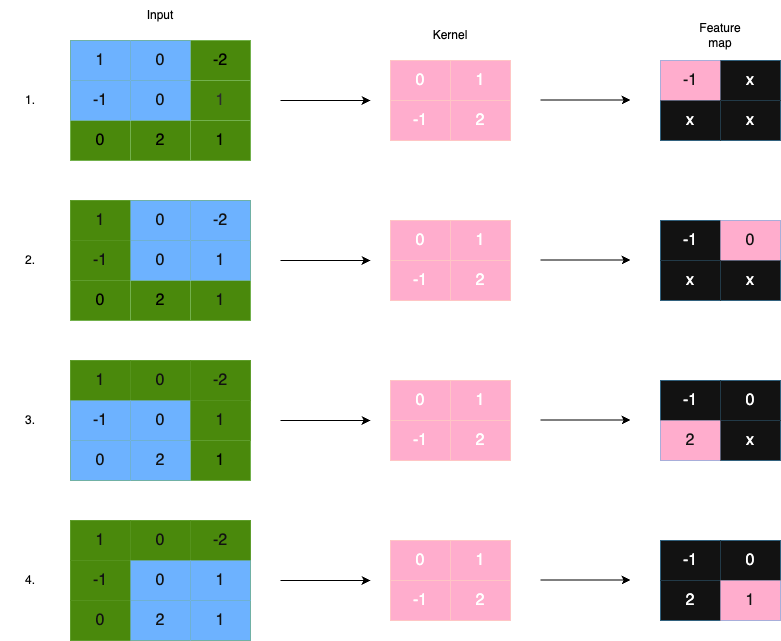
\includegraphics[width=0.8\textwidth]{Images/convolutional_operation.png}
  \caption{Illustration of the convolutional operation using a kernel on 2D input data.}
  \label{fig:convolution-diagram}
\end{figure}

\begin{definition}
  A \textit{Convolutional Neural Network (CNN)} \autocite{oshea2015introductionconvolutionalneuralnetworks} \autocite{jmse9040397} \autocite{LIU201711} is a discriminative deep learning model whose architecture is inspired by the hierarchical organization of the visual cortex in animals. CNNs are particularly effective in tasks involving image and spatial data processing due to their ability to capture local patterns and spatial hierarchies.

  The core components of a CNN are \textbf{convolutional layers} and \textbf{sub-sampling (pooling) layers}.

  \textbf{Convolutional layers} apply a set of learnable kernels (filters), each with its own weights, which slide over the input matrix to perform convolution operations. These layers extract local features by emphasizing patterns such as edges, textures, or more complex structures as the network deepens. They also preserve the spatial relationship between features, allowing the network to learn spatial hierarchies.

  \textbf{Sub-sampling layers}, also known as pooling layers, are used to progressively reduce the spatial dimensions of the feature maps. This helps decrease the computational complexity, control overfitting, and enhance the model’s invariance to small translations in the input. Common pooling operations include max pooling and average pooling, where the most prominent or average feature within a local region is retained. It's generally advised to use kernel size of 3 or less in pooling layers, due to their destructive nature and high chance of losing meaningful features.
\end{definition}

The concept of CNNs was inspired by Time-Delay Neural Networks, where weights are shared through time dimension. In CNNs weights are compacted into it's kernels. This architectural property vastly reduces the number of parameters and complexity of the network compared to Fully Connected Networks. CNNs are valued for their ability to learn to identify features without human interaction and for their empirically proven performance in processing multidimensional data with grid-like topology, like images and videos.

\section{Regularization}

\begin{definition}
  \textbf{Overfitting} \autocite{oshea2015introductionconvolutionalneuralnetworks} occurs when a model learns the details and noise in the training data to the extent that it negatively impacts the model’s performance on new, unseen data. This results in a model that has high accuracy on the training set but poor generalization to test data. Usually overfitting is indicated by model's performance on training dataset being much better then on test dataset \autocite{9944190}.
\end{definition}

Convolutional Neural Networks, despite their powerful feature extraction capabilities, are highly prone to overfitting (especially when trained on limited or imbalanced datasets) \autocite{alzubaidi2021review}. This is largely due to their large number of learnable parameters, which can easily adapt to noise in the training data. Regularization techniques are therefore essential to improve generalization and ensure that the model performs well on unseen data. Common methods include dropout, weight decay (L2 regularization), data augmentation, and early stopping. These techniques help constrain the learning process, reduce model complexity, and encourage the network to learn more robust and transferable features.

\begin{itemize}
  \item \textbf{Dropout:} \autocite{10.5555/2627435.2670313} A regularization technique where neurons are randomly deactivated during each training iteration. This prevents co-adaptation of neurons, encourages redundancy in feature learning, and improves generalization. During inference, the full network is used without dropout.

  \item \textbf{Data Augmentation:} \autocite{10.1145/3510413} Increases the size and diversity of the training dataset by applying transformations such as rotation, scaling, or flipping. This helps prevent overfitting and improves the model's ability to generalize.

  \item \textbf{Batch Normalization:} \autocite{NEURIPS2018_36072923} \autocite{10.1145/3510413} Normalizes layer outputs to have zero mean and unit variance. It reduces internal covariate shift, stabilizes training, and speeds up convergence by maintaining consistent activation distributions across training epochs. This normalization is applied to mini-batches during training and is often followed by a learnable scaling and shifting operation. By mitigating the shifting distributions of intermediate activations, batch normalization allows for higher learning rates, reduces sensitivity to initialization, and can also act as a form of regularization, sometimes reducing the need for dropout.

  \item \textbf{L1 and L2 Regularization:} \autocite{kukačka2017regularizationdeeplearningtaxonomy} These techniques add a penalty term to the loss function to discourage large weights and reduce the complexity of the model. L1 regularization (lasso) promotes sparsity by adding the absolute values of weights, and is represented by the term:
    \[
      \mathcal{L}_{L1} = \lambda \sum_{i} |w_i|
    \]
    where \( \lambda \) is the regularization strength and \( w_i \) are the model weights. L2 regularization (ridge) penalizes the squared values of weights, leading to smaller but non-zero weights, and is given by:
    \[
      \mathcal{L}_{L2} = \lambda \sum_{i} w_i^2
    \]
    The total loss function typically combines both the original loss and the regularization terms:
    \[
      \mathcal{L}_{total} = \mathcal{L}_{data} + \mathcal{L}_{L1} \text{ or } \mathcal{L}_{L2}
    \]
\end{itemize}

\section{Optimization}

\begin{definition}
  \textit{Gradient Descent} \autocite{sun2020optimization} \autocite{ruder2017overviewgradientdescentoptimization} is an iterative optimization algorithm used to minimize a loss function \( F(\theta) \) by updating the model parameters \( \theta \) in the direction of the negative gradient of the function. The basic update rule for gradient descent is given by
  \[
    \theta = \theta - \eta \nabla_\theta F(\theta),
  \]
  where \( \eta \) is the step size (also known as the learning rate), and \( \nabla_\theta F(\theta) \) is the gradient of the loss function.
\end{definition}

There are 3 variants of Gradient Descent: \autocite{ruder2017overviewgradientdescentoptimization}
\begin{itemize}
  \item \textit{Batch Gradient Descent} Computes gradient for the whole dataset and performs the parameter update only afterwards. Since the gradient is calculated only once per epoch, Batch Gradient Descent can be very slow and is not suitable for large datasets that don't fit into memory.
    \begin{algorithm}
      \caption{Gradient Descent}
      \begin{algorithmic}[1]
        \Require Number of epochs $N$, learning rate $\eta$, initial parameters $\theta$, loss function $L$, dataset $D$
        \Ensure Updated parameters $\theta$
        \For{$i = 1$ \textbf{to} $N$}
        \State $g \gets \text{evaluate\_gradient}(L, D, \theta)$
        \State $\theta \gets \theta - \eta \cdot g$
        \EndFor
      \end{algorithmic}
    \end{algorithm}
  \item \textit{Stochastic Gradient Descent (SGD)} calculates gradient and performs parameter update for each datapoint in the dataset. SGD is usually much faster and can be used in an online learning. But performing frequent updates with high variance usually leads to fluctuations in the objective function. These fluctuations usually help SGD find potentially more effective local minima in comparison to Batch Gradient Descent.
    \begin{algorithm}
      \caption{Stochastic Gradient Descent (SGD)}
      \begin{algorithmic}[1]
        \Require Number of epochs $N$, learning rate $\eta$, dataset $D$, initial parameters $\theta$, loss function $L$
        \Ensure Updated parameters $\theta$
        \For{$i = 1$ \textbf{to} $N$}
        \State Shuffle dataset $D$
        \ForAll{example $x$ in $D$}
        \State $g \gets \text{evaluate\_gradient}(L, x, \theta)$
        \State $\theta \gets \theta - \eta \cdot g$
        \EndFor
        \EndFor
      \end{algorithmic}
    \end{algorithm}
  \item \textit{Mini-Batch Gradient Descent} splits the data into mini-batches and calculates the gradient and updates the parameters for each batch separately. This way, it is able to reduce variance of parameter updates and take advantage of fast matrix operations that can be performed for the whole mini-batch at a time on modern Graphics Processing Units (GPUs).
    \begin{algorithm}
      \caption{Mini-Batch Gradient Descent}
      \begin{algorithmic}[1]
        \Require Number of epochs $N$, learning rate $\eta$, dataset $D$, batch size $b$, initial parameters $\theta$, loss function $L$
        \Ensure Updated parameters $\theta$
        \For{$i = 1$ \textbf{to} $N$}
        \State Shuffle dataset $D$
        \ForAll{batch $B$ in $\text{get\_batches}(D, b)$}
        \State $g \gets \text{evaluate\_gradient}(L, B, \theta)$
        \State $\theta \gets \theta - \eta \cdot g$
        \EndFor
        \EndFor
      \end{algorithmic}
    \end{algorithm}
\end{itemize}

\begin{definition}
  \textit{Backpropagation} \autocite{sun2020optimization} is an efficient algorithm for computing the gradient of the loss function with respect to the parameters of a neural network. Backpropagation systematically applies the chain rule of calculus layer by layer, propagating gradients backward from the output to the input to compute \( \nabla_\theta F(\theta) \) efficiently. From an optimization perspective, it enables the application of gradient-based methods, such as gradient descent, to train multi-layer networks.
\end{definition}

\begin{definition}
  \textit{Gradient Explosion/Vanishing} \autocite{sun2020optimization} refers to a common difficulty encountered when training deep neural networks, where gradients become either excessively large or exceedingly small as they are propagated backward through the network during training. From a signal processing perspective, gradient descent acts as a feedback correction mechanism: errors computed at the output layer are backpropagated through the network to update the weights of earlier layers. As this error signal passes through many layers, it may be repeatedly amplified (leading to gradient explosion) or attenuated (resulting in gradient vanishing). In either case, the learning process becomes unstable or stalls, preventing effective weight updates and model convergence.
\end{definition}

\begin{definition}
  \textit{Convergence} \autocite{sun2020optimization} in the context of optimization algorithms, particularly gradient descent, typically refers to the behavior where the sequence of iterates $\{\theta_t\}$ approaches a limit point as $t \rightarrow \infty$. A common formal criterion is that every limit point is a stationary point \autocite{bertsekas1997nonlinear}, meaning that the gradient vanishes at those points: $\nabla_\theta F(\theta^*) = 0$. However, this does not guarantee convergence to a global minimum and allows for several undesirable outcomes, such as the sequence having multiple limit points, or the sequence diverging with no limit points.
\end{definition}

\subsection{Optimization algorithms}
\begin{itemize}
  \item \textbf{Momentum} \\
    SGD struggles to find the right gradient direction when updates in one dimension are much steeper than in another \autocite{sutton1986two}. Momentum is a method that helps SGD overcome local minima faster and more effective. It works by updating the gradient vector $ v_t = \gamma v_{t-1} + \eta \nabla_\theta F(\theta) $ on each timestamp $t$ and updating the parameters using this vector $ \theta = \theta - v_t $. This ensures that the previous gradient directions are taken into account and helps the objective function accelerate in the right direction. The momentum term $\gamma$ is usually set to $0.9$ so that the momentum doesn't grow into infinity.
  \item \textbf{Nesterov accelerated gradient (NAG)} \autocite{nesterov1983method} \\
    The main problem with momentum is that it takes into account only previous vectors and doesn't react fast enough to the changes in the current and future gradient if the momentum is high enough. In NAG the next parameter update is approximated by subtracting the previous momentum. This way, the objective function slows down before the slopes and continues accelerating on the steep areas. The update vector for the current timestamp $t$ is calculated like this: $ v_t = \gamma v_{t-1} + \eta \nabla_\theta F(\theta - \gamma v_{t-1}) $.
  \item \textbf{Adagrad} \autocite{duchi2011adaptive} \\
    In this approach the learning rate is adapted for each parameter individually. Previously, the updates were performed for all parameters $\theta$ since each individual parameter $\theta_i$ used the same learning rate $\eta$. In Adagrad the gradient is calculated for each timestamp and for each parameter individually:
    \[ g_{t,i} = \nabla_\theta F(\theta_{t,i}) \]
    The update rule also changes. learning rate for each individual parameter now depends on the previous updates of this parameter:
    \[ \theta_{t+1, i} = \theta_{t, i} - \frac{\eta}{\sqrt{G_{t, ii} + \epsilon}} g_{t,i}, \]
    where $ G_t \in \mathbb{R}^{d \times d} $ is a diagonal matrix with each element $i, i$ being the sum of the squares of the gradients w.r.t. $ \theta_i $ up to timestamp $t$.
  \item \textbf{Adadelta} \autocite{zeiler2012adadeltaadaptivelearningrate} \\
    By accumulating the gradient updates, future learning rate eventually becomes very small in Adadelta. One way to eliminate this issue would be to take into account a fixed number of gradient updates for the diagonal matrix. In Adadelta the matrix $ G_t $ is replaced with the running average $E[g^2]_t = \gamma E[g^2]_{t-1} + (1 - \gamma)g_t^2$. Thus the formula for parameter update becomes:
    \[ \theta_{t+1, i} = \theta_{t, i} - \frac{\eta}{\sqrt{E[g^2]_t + \epsilon}} g_{t,i}, \]
  \item \textbf{Adam} \autocite{kingma2015adam} \\
    This method computes adaptive learning rates, just as Adadelta. The difference is that it calculates the estimates of the mean $ m_t = \beta_1 m_t + (1 - \beta_1)g_t $ and the uncentered variance $ v_t = \beta_2 v_{t-1} + (1 - \beta_2)g_t^2 $ of the gradient to determine the learning rates of the parameters:
    \[ \theta_{t+1} = \theta_t - \frac{\eta}{\sqrt{v_t} + \epsilon} m_t, \]
    The best default values are $0.9$ for $\beta_1$, $0.999$ for $\beta_2$ and $10^{-8}$ for $\epsilon$. Adam is one of the most popular GD algorithms with empirically proven efficiency.
  \item \textbf{Adamax} \autocite{kingma2015adam} \\
    The authors of adam note that it's update rule scales the gradient inversely proportional to a $L^2$ norm of their current and past gradients. After generalizing the $L^2$ to $L^p$ and letting $p \rightarrow \infty$, they're able to replace the term $\sqrt{v_t} + \epsilon$ with $u_t = max(\beta_2 * u_{t - 1}, |g_t|)$, thus receiving:
    \[ \theta_{t+1} = \theta_t - \frac{\eta}{u_t} m_t, \]
\end{itemize}
\subsection{Weights initialization}
% TODO: finish these sections